\documentclass[russian,utf8,pointsection]{eskdtext}
\usepackage{cmap}			% Поиск по русским словам в конечном pdf документе
\usepackage{eskdchngsheet}
\usepackage[T2A]{fontenc}
\usepackage{pscyr}			% Подключение "красивых" шрифтов киррилицы
\usepackage{amstext}
\usepackage{amsmath}
\usepackage{listings}

\usepackage{listings}		
\lstset{ %
	language=tcl,           % Язык программирования 	
	frame=single,           % Добавить рамку
	breaklines=true,        % Автоматический перенос строк
	breakatwhitespace=true, % Переносить строки по словам
	title=\lstname 
}

% работа с сылками
\usepackage{hyperref}
\usepackage[usenames,dvipsnames,svgnames,table,rgb]{xcolor}
\hypersetup{			
	unicode=true,           				% русские буквы в раздела PDF
	pdftitle={Заголовок},   				% Заголовок
	pdfauthor={Автор},      				% Автор
	pdfsubject={Тема},      				% Тема
	pdfcreator={Создатель}, 				% Создатель
	pdfproducer={Производитель}, 			% Производитель
	pdfkeywords={keyword1} {key2} {key3}, 	% Ключевые слова
	colorlinks=true,      					% false: ссылки в рамках; true: цветные ссылки
	linkcolor=NavyBlue,        				% внутренние ссылки
	citecolor=black,        				% на библиографию
	filecolor=black,        				% на файлы
	urlcolor=black          				% на URL
}

% Дает доступ к командам:
% \MakeTextUppercase{} - сделать все символы заглавными
\usepackage{textcase} 

%Изменение отображения Содержания
%\makeatletter
%\renewcommand{\l@section}{\@dottedtocline{1}{0em}{1.25em}}
%\renewcommand{\l@subsection}{\@dottedtocline{2}{1.25em}{1.75em}}
%\renewcommand{\l@subsubsection}{\@dottedtocline{3}{2.75em}{2.6em}}
%\makeatother

% Работа с таблицами
% p{} - top align, m{} - middle align, b{} - bottom align
\usepackage{ltablex} 										% longtable с функциональностю tabularx
\usepackage{multirow} 										% Слияние строк в таблице
\renewcommand{\tabularxcolumn}[1]{>{\arraybackslash}m{#1}}	% выравнивание в ячейке таблицы по середине по вертикали
\newcolumntype{M}[1]{>{\centering \arraybackslash}m{#1}} 	% колонка с заданной шириной и выравниванием по центру
\newcolumntype{Z}{>{\centering \arraybackslash} X} 			% колонка с выравниванием по центру

% Добавлено отображение Города на Титульном листе
\renewcommand{\ESKDtheTitleFieldX}{Екатеринбург \\ \ESKDtheYear}

% Уменьшен размер шрифта для заголовков секций
\ESKDsectStyle{section}{\large \bfseries \MakeTextUppercase}

% Выравнивание по центру.
% Предназначено для выравнивания надписей в шапке таблицы
\newcommand{\calign}[1]{\centering #1 \arraybackslash} 

%%% Работа с картинками
\usepackage{graphicx}  			% Для вставки рисунков
\graphicspath{{OrCAD/images/}}  % папки с картинками
\setlength\fboxsep{3pt} 		% Отступ рамки \fbox{} от рисунка
\setlength\fboxrule{1pt} 		% Толщина линий рамки \fbox{}
\usepackage{wrapfig} 			% Обтекание рисунков и таблиц текстом
\usepackage{float}

%%% Информация
\newcommand{\info}[1]{ %
\begin{flushleft}%
	\begin{tabular*}{\linewidth}{m{0.05\linewidth}m{0.9\linewidth}}%
		
\includegraphics[width=\linewidth]{info.jpg} & \textcolor{ForestGreen}{\textit{#1}}
	\end{tabular*}	
\end{flushleft}	
}



% Заполнение граф Титульного листа и основной надписи
\ESKDcompany{ООО <<Прософт-Системы>>}
%\ESKDclassCode{}
\ESKDtitle{OrCAD 16.6}
\ESKDdocName{Заметки}
\ESKDsignature{Заметки OrCAD 16.6 }
\ESKDgroup{\normalsize ООО <<Прософт-Системы>>}

% основная надпись
\ESKDauthor{\ESKDfontII Щеблыкин М.В.}
%\ESKDchecker{\ESKDfontII Макаров Е.Г.}
%\ESKDnormContr{\ESKDfontII Бунина О.Ю.}
%\ESKDapprovedBy{\ESKDfontII Чирков А.Г.}
\ESKDdate{2014/08/14}
%\ESKDcolumnI{АВАНТ К400 \\ \vspace{0.5cm} \ESKDfontIII{Инструкция по использованию протокола MODBUS}}


\begin{document}
\maketitle
\tableofcontents
	
\section{Design Entry CIS} \label{sec:cis}



%%------- Файл настроек Capture.ini
\subsection{Настройка} \label{ssec:cis_setup}


%%%------- Файл настроек Capture.ini
\subsubsection{Файл настроек Capture.ini} \label{sssec:cis_setup_capture_ini}

В~версии~\textbf{16.6} при~загрузке \textbf{Design Entry CIS} в~консоли выводится путь к~этому файлу. В~\textbf{16.5} "--- лежит в~\textit{<<../SPB\_16.5/tools/capture/>>}. 

Для~корректной работы \textbf{БД} необходимо заполнить в~файле настроек \textbf{Captrue.ini} параметры приведенные в~таблице~\ref{tab:capture_ini}.

\begin{tabularx}{\linewidth}{| m{6.5cm} | X |}
	\caption{Параметры \textit{Capture.ini}} \label{tab:capture_ini} \\
	\hline	
	\calign{Название} 		& \calign{Описание} 					\\ \hline
	\endfirsthead
	
	\multicolumn{2}{r}{продолжение следует\ldots} 
	\endfoot
	\endlastfoot
	
	\multicolumn{2}{l}{Продолжение таблицы~\ref{tab:capture_ini}} 					\\ \hline 
	\calign{Название} 		& \calign{Описание} 					\\ \hline
	\endhead
	
	[Allegro Footprints]	& Пути к~посадочным местам и контактным площадкам. Необходимо для работы \textit{Footprint Viewer}.  Например: \textit{<<Dir0=C:/..>>, <<Dir1=C:/..>>}.	\\ \hline
	[Footprint Viewer Type]	& Тип просмотрщика. Для отображения посадочных мест необходимо прописать \textit{Type=Allegro}.	\\ \hline
	[Part Library Directories]	& Пути к~библиотекам \textbf{УГО}. Например: \textit{<<Dir0=C:/..>>, <<Dir1=C:/..>>}.	\\ \hline
	[CIS Browse Directories]& Пути к~файлам документации. Позволяют в~\textbf{БД} указывать только имя файла, а~не~полный путь к~нему. Например: \textit{<<Dir0=C:/..>>, <<Dir1=C:/..>>}.	\\ \hline
	[Preferences]			& Для отключения автозагрузки стартовой страницы, необходимо прописать \textit{EnableStartPage=False}. Эту страницу можно загрузить вручную \textit{Accessories -> Cadence Tcl\textbackslash Tk Utilities -> Start page}. \\ \hline
\end{tabularx}



%%%------- Preferences
\subsubsection{Preferences}

На вкладке \textit{<<Colors/Print>>} можно задать цветовую палитру проекта и элементы выводимые на печать (\textit{checkbox}).

На вкладке \textit{<<Grid Display>>} можно настроить типа видимости сетки в редакторе схем (\textit{<<Schematic Page Grid>>}) и редакторе символов (\textit{<<Symbol Grid>>}). \textit{<<Grid spacing>>} отвечает за дробление сетки относительно шага ножек  и лучше эту опцию оставлять по умолчанию \textit{1/1}. \textit{<<Pointer snap to grid>>} отвечает за привязку к сетке: \textit{<<Fine>>} "--- без привязи, \textit{<<Master>>} "--- рекомендовано.

На вкладке \textit{<<Pad and Zoom>>} параметр \textit{<<Auto Scroll Percent>>} рекомендуется установить 2.

На вкладке \textit{<<Miscellaneous>>} параметр \textit{<<Intertool Communication>>} отвечает за интерактивную связь редактора схем и плат. А параметр \textit{<<Wire Drag>>} отвечает за возможность перемещения элемента вместе с линиями связи.



%%%------- Preferences
\subsubsection{Design Template}

На вкладке \textit{<<Page Size>>} параметр \textit{<<Pin-to-Pin Spacing>>} отвечает за шаг ножек символа.



%%------- База данных
\newpage
\subsection{База данных} \label{ssec:bd}

Для корректной работы \textbf{БД} необходимо настроить \hyperref[sssec:cis_setup_capture_ini]{\textbf{Capture.ini}}.

Значения для \textbf{multi-values} полей записывают через запятую.

%%%------- Рекомендации по заполнению
\subsubsection{Рекомендации по заполнению} \label{sssec:bd_contet}
В таблице \ref{tab:bd_content} описаны поля, которые рекомендованы для заполнения в~каждой таблице \textbf{БД}.

\begin{tabularx}{\linewidth}{| m{4cm} | X |}
	\caption{Обязательные поля \textbf{БД}} \label{tab:bd_content} \\
	\hline	
	\calign{Название} 		& \calign{Описание} 					\\ \hline
	\endfirsthead
	
	\multicolumn{2}{r}{продолжение следует\ldots} 
	\endfoot
	\endlastfoot
	
	\multicolumn{2}{l}{Продолжение таблицы~\ref{tab:bd_content}} 	\\ \hline 
	\calign{Название} 		& \calign{Описание} 					\\ \hline
	\endhead
	
	Part Number				& Уникальное имя элемента. Ключевое поле, поэтому повторы не~допускаются. Использовать русские символы нельзя.	\\ \hline
	Value					& Значение компонента. Например: 1.0u, 10k. Использовать русские символы нельзя. Используется разделительная точка.	\\ \hline
	Description				& Наименование компонента передаваемое в~документацию.	\\ \hline
	Schematic Part			& УГО элемента. Можно просто вводить имя символа, например \textit{CAP\_P}. А~можно указать библиотеку источник, например \textit{DISCRETE/CAP\_P}. \textbf{multi-values} 	\\ \hline
	PCB Footprint			& Посадочное место. Название должно совпадать с~имеющимся файлом посадочного места. Например: \textit{CAPC2013X70N}. \\ \hline
	ALT\_SYMBOLS			& Дополнительное посадочное место. Например, можно использовать для резистора с~вертикальной и горизонтальной установкой или для посадочных мест разной точности. \textbf{multi-values}	\\ \hline
	Datasheet				& Интернет-ссылка на~описание элемента. \textbf{multi-values} 	\\ \hline
	Local Data				& Ссылка на~локальный документ. Можно прописывать как полный путь, так~и просто имя файла, который в~дальнейшем будет искаться в~прописанных путях. \textbf{multi-values}	\\ \hline
	Part Tye				& Тип компонента. Например: \textit{Chip\textbackslash0805}. Рекомендуемые обозначения приведены в~таблице~\ref{tab:app_bd_part_type} приложения~\ref{app:bd}.	\\ \hline
	NC						& Пины отсутствующие на~УГО символа, но~имеющиеся на~посадочном месте. Например: 1,2.	\\ \hline
	Code 1C					& Код элемента в~\textbf{базе 1С} предприятия.	\\ \hline
	Case					& Корпус элемента, передаваемый в~документацию. Например: \textbf{SOIC\_16}. Рекомендуемые обозначения приведены в~таблице \ref{tab:app_bd_case} приложения \ref{app:bd}.	\\ \hline
	Comment					& Дополнительная информация о~элементе. Например, вариант установки для~выводных резисторов.	\\ \hline
\end{tabularx}



%%%------- Регистрация в системе
\subsubsection{Регистрация в системе} \label{sssec:bd_install}
Для того чтобы база стала видна из~схемного редактора, надо сначала настроить систему. Для этого необходимо обладать правами Администратора:
\begin{enumerate}
	\item В \textbf{Windows XP}: \textit{<<Пуск / Настройка / Панель управления / Администрирование / Источники данных ODBC>>}.
	
	В \textbf{Windows 7}: \textit{<<Windows / system32 / odbcad32.exe>>}, из \textit{<<Выполнить>>} не работает! 
	
	\begin{figure}[H]
		\center{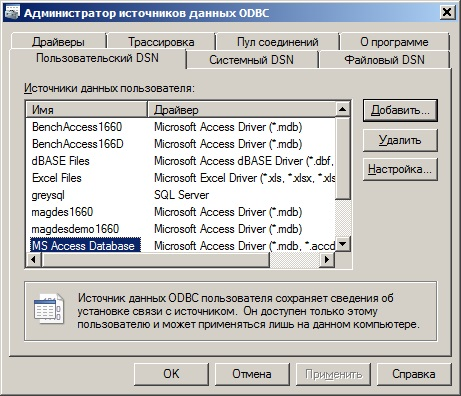
\includegraphics[width=0.5\linewidth]{bd_odbc_1.jpg}}
	\end{figure}
	
	\item Жмем \textit{<<Добавить>>} и выбираем драйвер \textit{<<Microsoft Access Driver (*.mdb, *accdb)>>}.
	
	\begin{figure}[H]
		\center{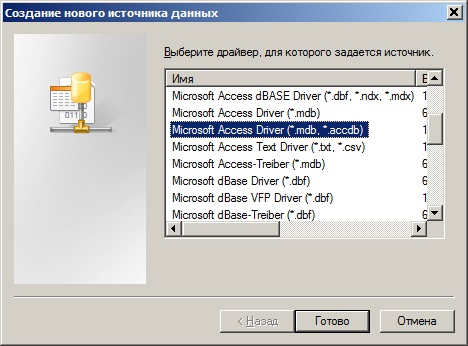
\includegraphics[width=0.5\linewidth]{bd_odbc_2.jpg}}
	\end{figure}
	
	\info{ Если данный пункт отсутствует, необходимо установить \textbf{Microsoft Access}.}
	
	\item Жмем \textit{<<Готово>>}, в~открывшейся форме выбираем необходимую \textbf{БД} и заполняем поля.
	
	\begin{figure}[H]
		\center{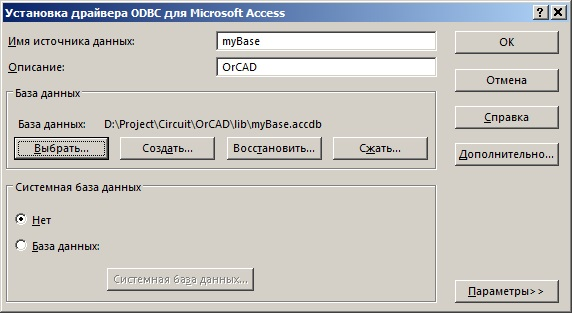
\includegraphics[width=0.5\linewidth]{bd_odbc_3.jpg}}
	\end{figure}
	
	\item Жмем \textit{<<OK>>} и проверяем что база появилась в списке.
\end{enumerate}



%%%------- Настройка multi-values полей
\subsubsection{Настройка multi-values полей} \label{sssec:bd_multi_value}

Начиная с версии \textbf{16.6}, каждое поле \textbf{БД} может являться \textbf{multi-values}, т.е. можно записывать несколько значений.

Для этого необходимо поместить в автозагрузку скриптов: \\
\textit{C:/SPB\_Data-Silent/cdssetup/OrCAD\_Capture/tclscripts/capAutoLoad} или \\
\textit{C:/Cadence/SPB\_16.6/tools/capture/tclscripts/capAutoLoad}), \\
файл \textit{*.tcl} со следующим содержимым:
\lstinputlisting[language=tcl]{OrCAD/CISRowColor.tcl}	% листинг файла

В примере выше, \textbf{multi-values} параметром объявляется \textit{<<Local Data>>}. Добавление других параметров осуществляется там же, например: 
\begin{center}
	\textit{SetCISMultiValuedField \{Datasheet\}}
\end{center}



%%%------- Подключение в CIS
\subsubsection{Подключение в CIS} \label{sssec:bd_setup_cis}

Подключение зарегистрированной в~системе \hyperlink{sssec:bd_install}{\textbf{БД}} происходит в~несколько шагов:
\begin{enumerate}
	\item Запустить \textbf{Design Entry CIS};
	\item Создать новый проект или открыть имеющийся;
	\item Перейти в окно \textit{<<Menu -> Options -> CIS Configuration\ldots>>};
		\begin{figure}[H]
			\center{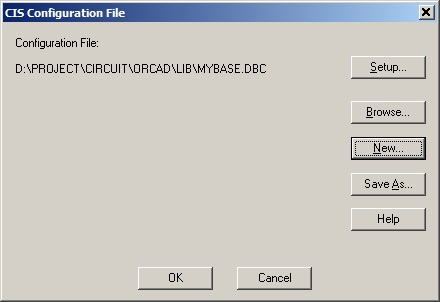
\includegraphics[width=0.6\linewidth]{bd_setup_1.jpg}}
		\end{figure}
	\item Перейти в окно создания нового подключения \textit{<<New\ldots>>};
	\item Выбрать из списка нужную базу;
	\item \label{l:1} Выбрать нужные таблицы; 
		\begin{figure}[H]
			\center{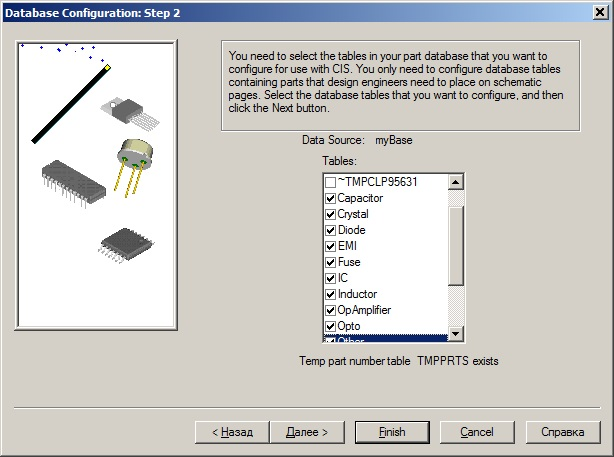
\includegraphics[width=0.6\linewidth]{bd_setup_2.jpg}}
		\end{figure}
	\item Выбрать соответствие между полями таблицы и параметрами \textbf{CIS};
		\begin{figure}[H]
			\center{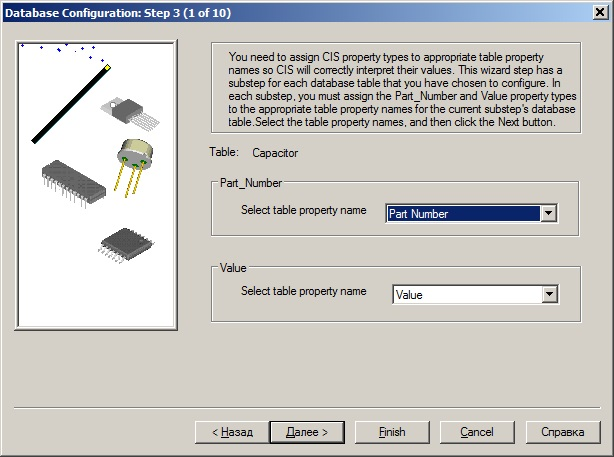
\includegraphics[width=0.6\linewidth]{bd_setup_3.jpg}}
		\end{figure}
		\info{Поля с одинаковыми именам заполняются автоматически.}
		\begin{figure}[H]
			\center{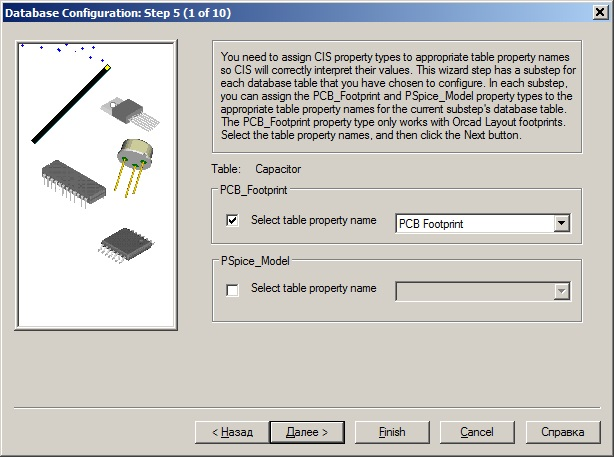
\includegraphics[width=0.6\linewidth]{bd_setup_4.jpg}}
		\end{figure}		
	\item Выбрать поля которые будут передаваться из БД в проект. Если \textbf{БД} заполнялась в соответствии с \hyperlink{sssec:bd_contet}{рекомендациями}, то как минимум должны быть отмечены: \textit{<<Value>>, <<PCB Footrpint>>, <<ALT\_SYMBOLS>>, <<NC>>, <<Description>>};
		\begin{figure}[H]
			\center{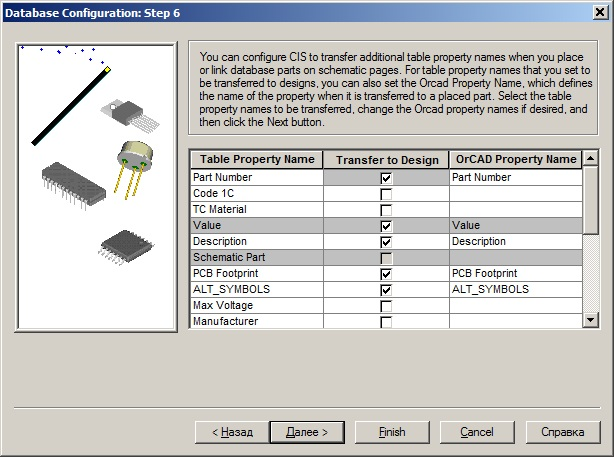
\includegraphics[width=0.6\linewidth]{bd_setup_5.jpg}}
		\end{figure}
	\item Если в дальнейшем планируется пользование \textbf{ICA}, то установить флаг \textit{<<ICA Properties>>}, иначе \textit{<<No ICA Properties>>};
		\begin{figure}[H]
			\center{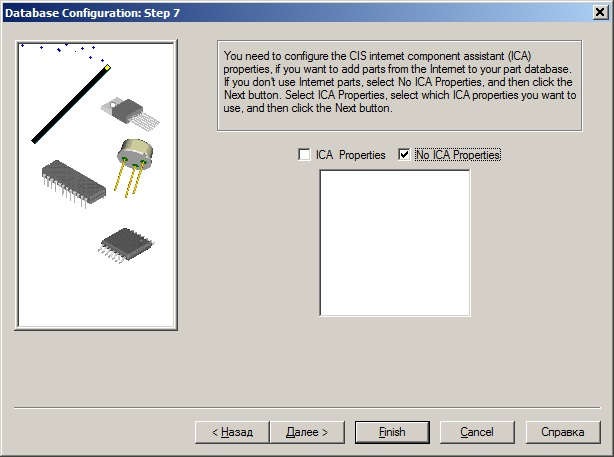
\includegraphics[width=0.6\linewidth]{bd_setup_6.jpg}}
		\end{figure}
	\item Выбрать какие параметры являются ссылками. Например: \textit{<<Datasheet>>} и \textit{<<Local Data>>};
		\begin{figure}[H]
			\center{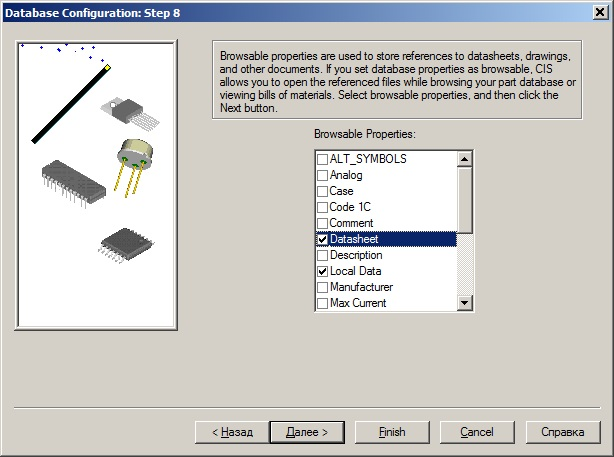
\includegraphics[width=0.6\linewidth]{bd_setup_7.jpg}}
		\end{figure}
	\item Выбрать параметры, которые будут видимы на схеме при установке элементов. Например: \textit{<<Part Number>>};
		\begin{figure}[H]
			\center{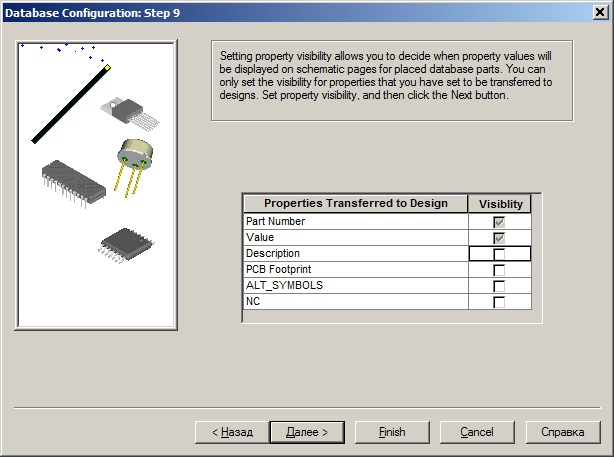
\includegraphics[width=0.6\linewidth]{bd_setup_8.jpg}}
		\end{figure}
	\item Выбрать ключевые поля
		\begin{figure}[H]
			\center{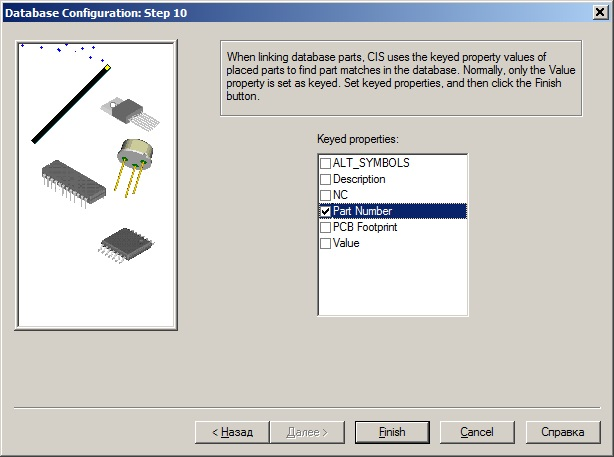
\includegraphics[width=0.6\linewidth]{bd_setup_9.jpg}}
		\end{figure}	
	\item В окне \textit{<<Configure Database>>} перейти на вкладку \textit{<<Administrative Preferences>>}. Снять флаги \textit{<<Allow Duplicate Part Numbers>>} и \textit{<<Assign Temportary Part Numbers Automatically>>}. В поле \textit{<<Delimiter for Multi-Values>>} ввести знак разделителя, который используется в \textbf{БД}. Если она заполнена согласно \hyperlink{sssec:bd_contet}{рекомендациям}, то это будет \textbf{запятая};
		\begin{figure}[H]
			\center{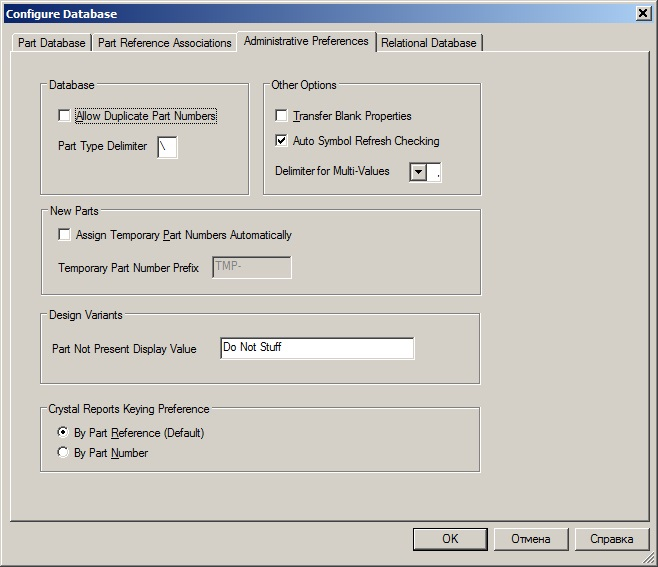
\includegraphics[width=0.6\linewidth]{bd_setup_10.jpg}}
		\end{figure}
	\item Во вкладке \textit{<<part Database>>} проверить настройки полей для каждой из таблиц и нажать \textit{<<OK>>}.
		\info{В дальнейшем вернуться в окно настроек \textit{<<Configure Database>>} можно так: \textit{<<Options -> CIS Configuration\ldots -> Setup>>}.}
		\begin{figure}[H]
			\center{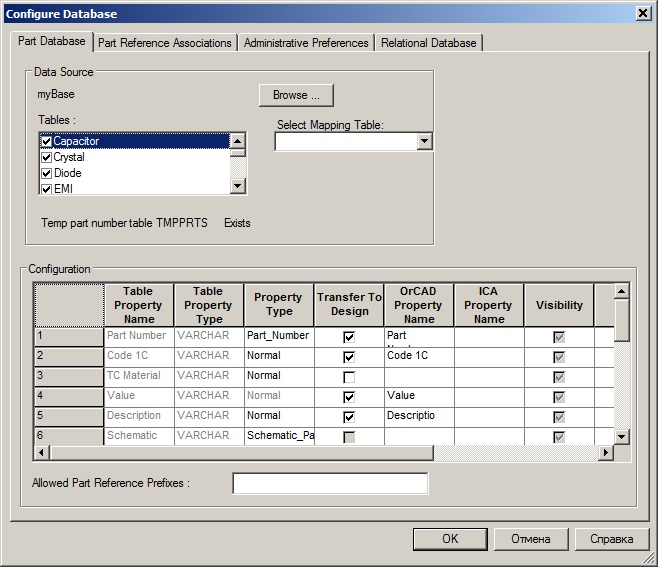
\includegraphics[width=0.6\linewidth]{bd_setup_11.jpg}}
		\end{figure}
	
\end{enumerate}



%%------- Создание символа УГО
\newpage
\subsection{Создание символа УГО} \label{ssec:create_symbol}

Пины \textit{<<Zero Length>>} обычно используются для силовых выводов, т.е. \textit{<<Power>>}.

%%%------- Стандартный способ
\subsubsection{Стандартный способ} \label{sssec:create_symbol_standart}

В окне проекта нажать \textbf{RMB} на нужной библиотеке и выбрать \textit{<<New Part>>}. Если необходим символ без привязки к физической реализации, вместо \textit{<<New Symbol>>} выбираем \textbf{<<New Symbol>>}, который позволяет определить следующие типы символов: \textit{<<Power>>, <<Off-Page Connector>>, <<Hierarchical Port>>, <<Title Block>> , <<Pin Shape>>}.

Переход между символами многосекционного УГО осуществляется при помощи \textit{<<Menu -> View -> Package>>} или кнопок \textbf{<<Ctrl+N>>} и \textbf{<<Ctrl+B>>}.

Таблицу настроек пинов можно вызвать из общего вида (\textit{<<Menu -> View -> Package>>}) \textit{<<Menu -> Edit -> Properties\ldots>>}. \textit{<<Pin Group>>} при этом обозначает эквивалентность выводов.
	\begin{figure}[H]
		\center{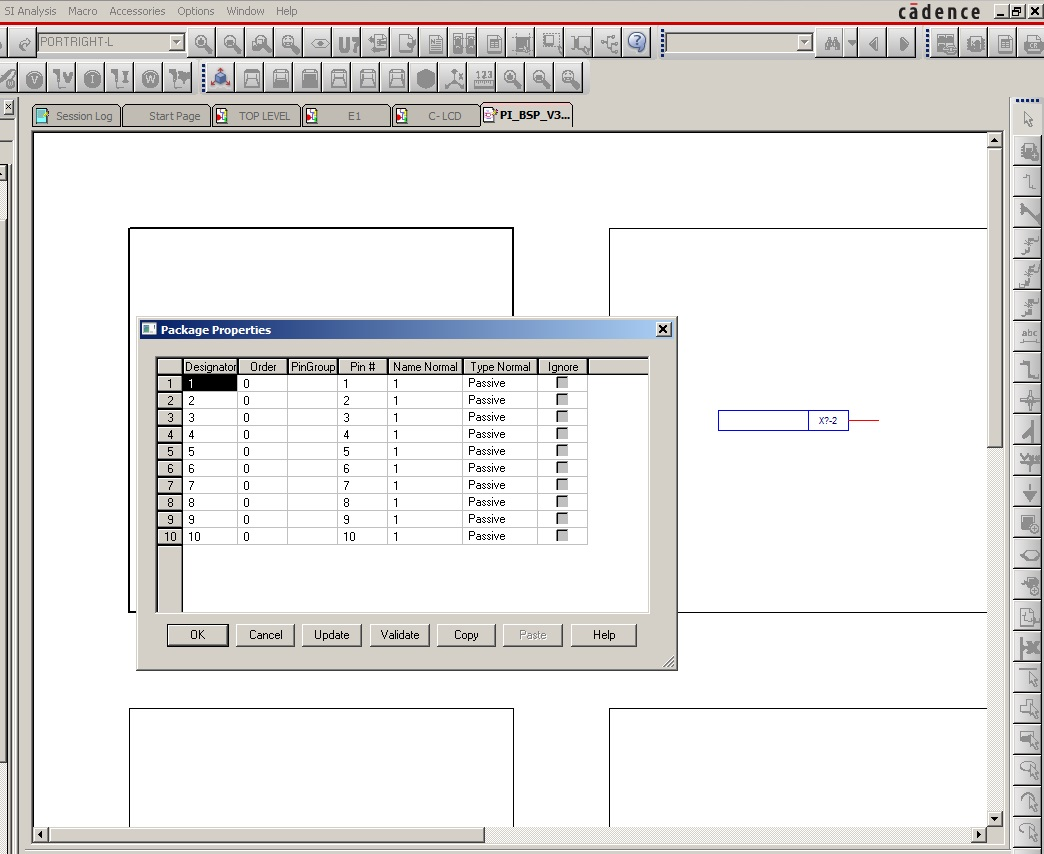
\includegraphics[width=0.6\linewidth]{create_symbol_1.jpg}}
	\end{figure}

%%%------- Табличный способ
\subsubsection{Табличный способ} \label{sssec:create_symbol_table}

В окне проекта нажать \textbf{RMB} на нужной библиотеке и выбрать \textit{<<New Part From Spreadsheet>>}.

Для изменения нескольких ячеек одновременно, надо удерживать \textbf{<<Shift>>}. 

Вернуться к таблице во время редактирования символа можно нажав \textbf{RMB} на элементе и выбрав \textit{<<Split Part>>}.
	\begin{figure}[H]
		\center{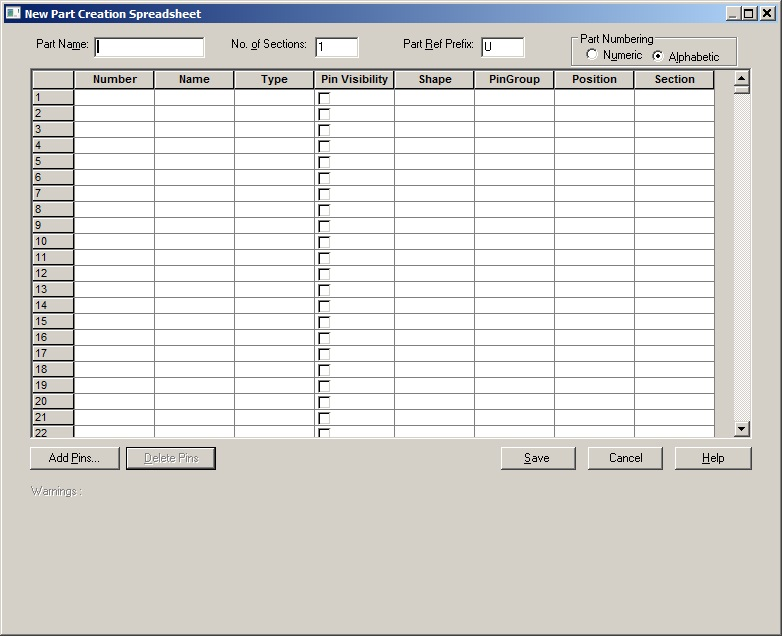
\includegraphics[width=0.6\linewidth]{create_symbol_2.jpg}}
	\end{figure}



%%%------- По данным из файла
\subsubsection{По данным из файла} \label{sssec:create_symbol_file}

При помощи данной опции можно создавать \textbf{УГО} по полученным из файла, созданным например для \textbf{ПЛИС} из проекта \textbf{Quartus}, данным.

В окне проекта перейти во вкладку \textit{<<Menu -> Tools -> Generate Part>>}. При первом создании установить флаг \textit{<<Create new part>>}, для обновления \textit{<<Update pins on existing part in library>>}.
	\begin{figure}[H]
		\center{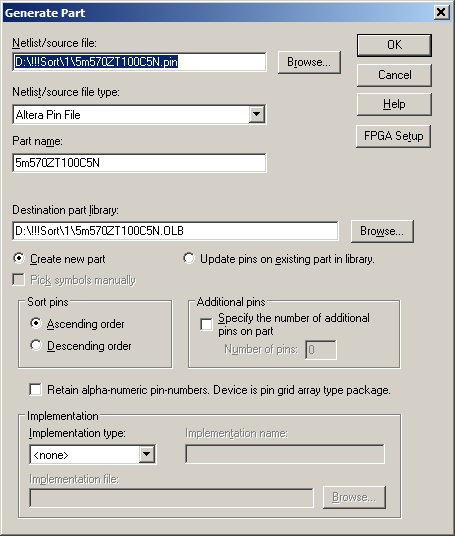
\includegraphics[width=0.6\linewidth]{create_symbol_3.jpg}}
	\end{figure}

При обновлении расположение выводов останется в соответствии с данными именами. 

Для удобства добавления дополнительных ножек, можно при создании символа зарезервировать несколько ножек в \textit{<<Additional pins>>}. Либо в последствии добавить на символ ножку с нужным именем и уже после этого переходить в \textit{<<Generate Part>>}. 

%%%------- По SPICE описанию
\subsubsection{По SPICE описанию} \label{sssec:create_symbol_spice}

% TODO

%%%------- Объединение ножек
\subsubsection{Дополнительные свойства символа} \label{sssec:create_symbol_spice}

Номера выводов \textbf{УГО} и их~количество на~схеме должны в~точности соответствовать его~посадочному месту. Иначе при~создании списка соединений будет сформирована ошибка. Но~иногда возникает желание скрыть несколько выводов подключенных к~одной цепи, либо избавиться от~не~используемых. Это можно сделать за~cчет использования дополнительных свойств символа \textit{NC} и \textit{PACK\_SHORT}.

Ниже приведено использование данных свойств на~основе элемента LM317.

Данная микросхема имеет 4~вывода~ $V_{OUT}$ 2, 3, 6, 7. Которые объединены друг с~другом. И два не~используемых вывода~\textit{NC} 4 и 5.
	\begin{figure}[H]
		\center{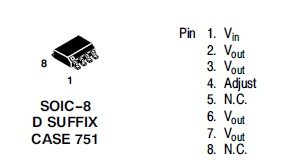
\includegraphics[width=0.6\linewidth]{lm317_pin.jpg}}
	\end{figure}
	
Необходимо получить символ на подобии этого]:	
	\begin{figure}[H]
		\center{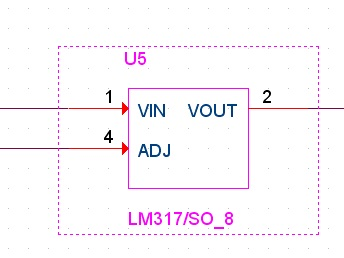
\includegraphics[width=0.5\linewidth]{lm317_symbol.jpg}}
	\end{figure}
	
Для начала, рисуется УГО со всеми используемыми выводами элемента. Все имена должны быть уникальными. Выводам с~одноименными названиями можно дать названия типа \textit{VOUT1} или \textit{VOUT\#3}, где после символа~\textit{\#} стоит номер вывода.
	\begin{figure}[H]
		\center{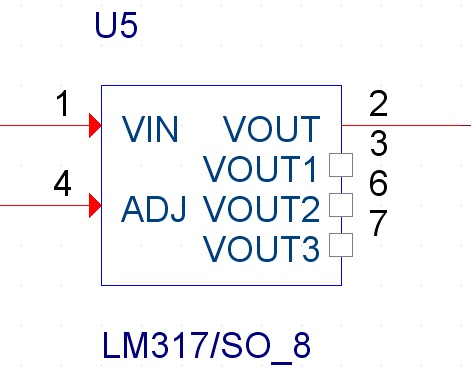
\includegraphics[width=0.4\linewidth]{lm317_symbol_1.jpg}}
	\end{figure}

Далее необходимо перейти в~окно редактирования свойств <<Options -> Part Properties...>>.
	\begin{figure}[H]
		\center{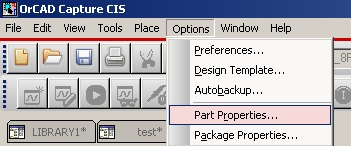
\includegraphics[width=0.6\linewidth]{lm317_part_properties.jpg}}
	\end{figure}

Добавить свойство \textit{PACK\_SHORT} и указать какие выводы должны быть объединены. 
	\begin{figure}[H]
		\center{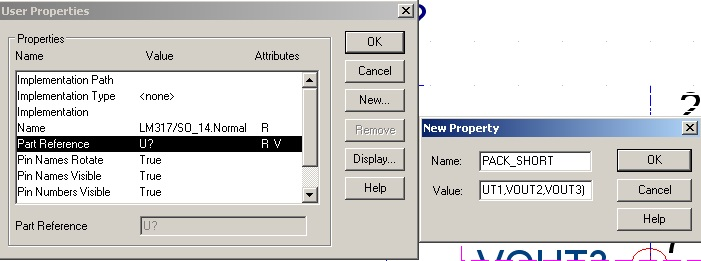
\includegraphics[width=\linewidth]{lm317_pack_short.jpg}}
	\end{figure}
Значение вводится в~ввиде:
	\begin{equation}
		PACK\_SHORT = (<group1>)(<group2>)[<group3>]
	\end{equation}
	\begin{ESKDexplanation}
		\item[,где] $<group>$ записывается в~ввиде $(logicPin1, logicPin2)$.
	\end{ESKDexplanation}
	
Далее необходимо сделать невидимыми нужные выводы.

Сначала выбрать \textit{<<View -> Package>>}:
	\begin{figure}[H]
		\center{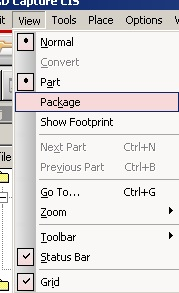
\includegraphics[width=0.25\linewidth]{lm317_view_package.jpg}}
	\end{figure}
, а затем \textit{<<Edit -> Properties...>>}. 
	\begin{figure}[H]
		\center{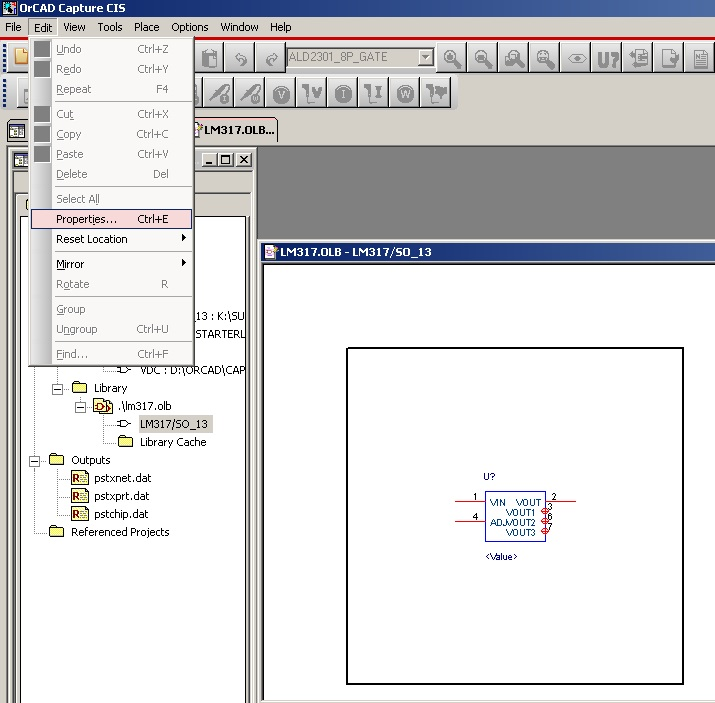
\includegraphics[width=0.6\linewidth]{lm317_edit_properties.jpg}}
	\end{figure}
И установить свойство выводов \textit{Ignore}.
	\begin{figure}[H]
		\center{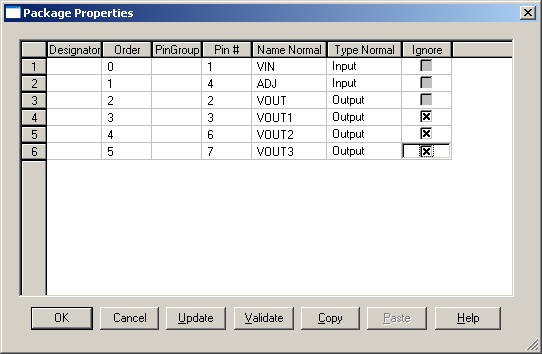
\includegraphics[width=0.6\linewidth]{lm317_package_properties.jpg}}
	\end{figure}
В~итоге будет получен желаемый результат.

Для того чтобы установить свойство \textit{NC}, необходимо перейти в~окно редактирования свойств <<Options -> Part Properties...>>.
	 \begin{figure}[H]
	 	\center{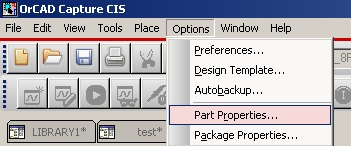
\includegraphics[width=0.6\linewidth]{lm317_part_properties.jpg}}
	 \end{figure}
И добавить свойство~\textit{NC} с~перечислением всех необходимых не~подключенных номеров выводов.
	\begin{figure}[H]
		\center{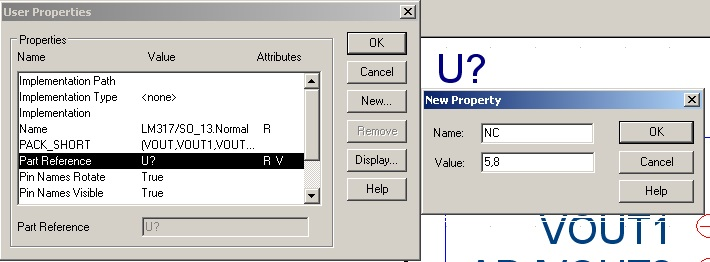
\includegraphics[width=0.8\linewidth]{lm317_nc.jpg}}
	\end{figure}

\info{Для передачи со~схемы символа без выводов на~разводку, например радиатора с~креплением к~плате, необходимо добавить свойство \textit{CLASS} со~значением \textit{MECHANICAL}.}  
	
%%-------
\newpage
\subsection{Вариантные исполнения} \label{ssec:variant_list}



%%%-------
\subsubsection{Передача в PCB Editor} \label{sssec:export_variant_list}

Передача вариантных исполнений из~схемного редактора в~редактор печатных плат, осуществляется в~несколько шагов:
\begin{enumerate}
	\item Запустить \textbf{Design Entry CIS};
	
	\item Перейти в~окно \textit{Part Manager};
	
	\item Сформировать список вариантных исполнений \textit{<<Menu -> Tools -> Export Variant List>>}; 
	
	\item Запустить \textbf{PCB Editor};
	
	\item Перейти в~окно \textit{<<Menu -> Manufacture -> Variants -> Create Assembly Drawing...>>};
	
	\item Выбрать нужные настройки и вариант исполнения.
	
		\begin{figure}[H]
			\center{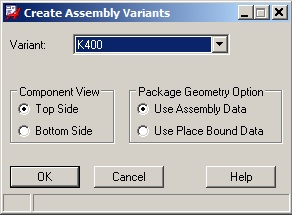
\includegraphics{create_assembly_variants.jpg}}
%			\caption{Окно вариантного исполнения} 
%			\label{fig:create_assembly_variants}
		\end{figure}	
	
\end{enumerate}

После этих действий появится новый подкласс в~классе \textit{Manufacture}. Для настроек установленных выше это будет \textit{<<Manufacture/K400\_Top>>}.


%%-------
\newpage
\subsection{Надстройки} \label{ssec:variant_list} \label{ssec:cis_plugin}



%%%-------
\subsubsection{Подключение} \label{sssec:cis_plugin_setup}

Для автоматической загрузки, необходимо разместить скачанные \textbf{tcl} скрипты в~папку \textit{<<\%CDS\_SITE\%/OrCAD\_Capture/tclscripts/capAutoLoad/>>}, либо создать там отдельную папку.

Для загрузки в ручную, необходимо разместить скачанные \textbf{tcl} скрипты в~папку \textit{<<\%CDS\_SITE\%/OrCAD\_Capture/tclscripts/>>}, либо создать там отдельную папку.




\section{PCB Editor} \label{sec:pcb_editor}



%%-------
\subsection{User Preferences} \label{ssec:user_preferences}

Опция параметра \textit{Effective} определяет точку применения: при активации, после рестарта, по~команде.

Опция параметра \textit{Favorite} позволяет добавить параметр на~вкладку избранное \textit{my\_favorites}.

\info{Приоритет поиска по~заданным в~параметрах путях "--- сверху вниз.}

\begin{tabularx}{\linewidth}{| m{6.5cm} | X |}
	\caption{Параметры \textit{User Preferences}} \label{tab:user_preferences} \\
	\hline	
	\calign{Название} 		& \calign{Описание} 					\\ \hline
	\endfirsthead
	
	\multicolumn{2}{r}{продолжение следует\ldots} 
	\endfoot
	\endlastfoot
	
	\multicolumn{2}{l}{Продолжение таблицы \ref{tab:user_preferences}} 					\\ \hline 
	\calign{Название} 		& \calign{Описание} 					\\ \hline
	\endhead
	
	\multicolumn{2}{|c|}{\textbf{Paths/Config}}						\\ \hline
	artpath					& Пути к~настройкам герберов.			\\ \hline
	viewpath				& Путь к~цветовым настройкам.			\\ \hline
	ncdpath					& Путь к~настройкам сверловки.			\\ \hline
	wizard\_template\_path	& Путь к~шаблонам ПП и символов (форм, механики, чертежей). \\ \hline
	
	\multicolumn{2}{|c|}{\textbf{Paths/Library}}					\\ \hline
	miscpath 				& Путь к~различным файлам, в~том~числе настройкам для экспорта в~*.dxf. \\ \hline
	modulepath 				& Путь к~смхемам повторного использования *.mdd. \\ \hline
	ncdpath 				& Путь к~настройкам сверловки.			\\ \hline
	padpath 				& Путь к~контактным площадкам.			\\ \hline
	parampath 				& Путь к~файлу настроек проекта (настройки цветов, сетки, трассировки). \\ \hline
	psmpath 				& Путь к~посадочным местам.				\\ \hline
	steppath 				& Путь к~3D~моделям.					\\ \hline
	techpath 				& Путь к~файлам технологических настроек (хранит также информацию о~слоях). \\ \hline
	topology\_template\_path& Путь к~файлам ограничений (материалы, проводимость). \\ \hline
	
	\multicolumn{2}{|c|}{\textbf{Другие}}									\\ \hline
	acon\_diag 				& Вне зависимости от~угла расположения элемента, трассировка начнется под~его углом. \\ \hline
	addline\_nomerge 		& Запрет связи двух линий при их соединении.	\\ \hline
	ads\_sdart 				& Путь для гербер файлов и файлов сверловки (по~умолчанию ложится в~проект). \\ \hline
	ads\_sdlog 				& Путь для log-файлов (по~умолчанию ложится в~проект). \\ \hline
	ads\_sdplot 			& Путь для plot файлов.					\\ \hline
	ads\_sdreport 			& Путь для отчетов.						\\ \hline
	allegro\_dynam\_timing	& \textcolor{red}{?!} 					\\ \hline
	allegro\_etch\_lenght\_on& Отображение текущей длинны проводника.\\ \hline
	autosave 				& Включение автосохранения.				\\ \hline
	autosave\_name			& Имя файла автосохранения.				\\ \hline
	autosave\_time			& Период автосохранения.				\\ \hline
	cancel\_key				& Клавиша полной отмены.				\\ \hline
	datatips\_delay 		& Задержка на~появление подсказки.		\\ \hline
	db\_tier\_nomsg 		& Сообщение об~ошибке версий БД.		\\ \hline
	dcnets\_delete\_norat	& Удаление свойства NO\_RAT для цепей питания.	\\ \hline
	disable\_opengl			& Отключение режима opengl.				\\ \hline
	display\_refdes\_rats	& Показывает привязку поз. обозначений.	\\ \hline
	draw\_etch\_outline		& Отображение границ линий.				\\ \hline
	dxf\_version			& Версия выходного *.dxf файла.			\\ \hline
	idf\_place\_bound\_bottom & \textcolor{red}{?!} 					\\ \hline
	idf\_place\_bound\_top	& \textcolor{red}{?!} 					\\ \hline
	idx\_place\_bound\_bottom & \textcolor{red}{?!} 				\\ \hline
	idx\_place\_bound\_top	& Слои для настройки высоты компонента.	\\ \hline
	logic\_edit\_enabled 	& Включение "Logic/Net logic" команд.	\\ \hline 
	lp\_abs\_origin			& Точка привязки для IPF файлов.		\\ \hline 
	max\_undo\_memory 		& Размер памяти отведенной под откаты.	\\ \hline
	modules\_no\_5x\_support& \textcolor{red}{?!}					\\ \hline
	nolast\_directory 		& \textcolor{red}{?!}					\\ \hline
	nolast\_file 			& \textcolor{red}{?!}					\\ \hline
	preserve\_symbol\_textblocks & \textcolor{red}{?!}				\\ \hline	
	step\_unsupported\_prototype & Включение опций поддержки 3D step-моделей. \\ \hline
%	symed\_pin\_names\_for\_voltage\_pins & \textcolor{red}{?!}		\\ \hline	
	undo\_depth 			& Количество откатов.					\\ \hline
	use\_accure\_delay\_calculation & Включение вычисления неравномерности экранирующего слоя. \\ \hline
\end{tabularx}



%%-------
\newpage
\subsection{3D модель} \label{ssec:3d_model}



%%%-------
\subsubsection{Привязка модели к посадочному месту} \label{sssec:step_package_mapping}

Подключить 3D модель, а~точнее STEP, к~посадочному месту можно выполнив следующие шаги:

\begin{enumerate}
	\item Скачать или создать STEP модель и~разместить ее по~доступному пути;
	\info{Доступный путь, это путь в~текущей папке символа или путь прописанный в~настройках \textit{<<User Preferences -> Paths -> Library -> steppath>>}.}
	
	\item Запустить \textbf{PCB Editor};
	
	\item Открыть файл посадочного места (*.dra) и~перейти в~окно \textit{<<Setup -> Step Package Mapping...>>};
	\info{Раньше этот пункт меню появлялся только после установки параметра \textit{<<step\_unsupported\_prototype>>} в~\textit{<<User Preferences>>}. В~версии \textbf{16.6 S032} такого параметра уже нет.}
	
	\item В~списке \textit{<<Available STEP Models>>} выбрать нужную модель элемента;
	
	\begin{figure}[H]
		\center{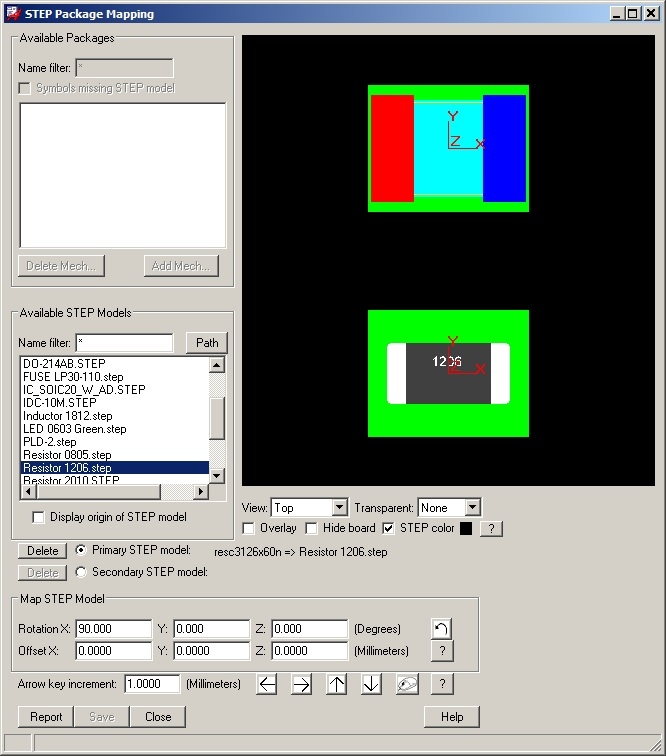
\includegraphics[width=0.5\linewidth]{step_model_mapping.jpg}}
%		\caption{Окно подключения \textbf{3D}~модели} 
%		\label{fig:step_model_mapping}
	\end{figure}
	
	\item При помощи поворотов и~сдвигов \textit{<<Map STEP Model>>} добиться нужного положения модели относительно контактных площадок. Правильность установки можно оценить переключая виды;
	\info{Посадочное место и~модель можно наложить друг на~друга, включив настройку \textit{<<Overlay>>}.}
	\info{Для удобства совмещения модели и~посадочного места, у~последнего точку привязки надо делать по~центру. По~крайней мере для многих моделей, что скачивал я, требовались лишь простейшие повороты, либо все сразу совпадало.} 
	\item Сохранить полученный результат. По~умолчанию это будет сделано в~\textit{<<./stepFaceFiles4Map/>>};
	
	\item В~дальнейшем при установке элемента на плату, он будет иметь 3D~изображение;
	
	\item В~итоге можно получить довольно приятную картинку платы, например как на~рисунке ниже.
	
	\begin{figure}[H]
		\center{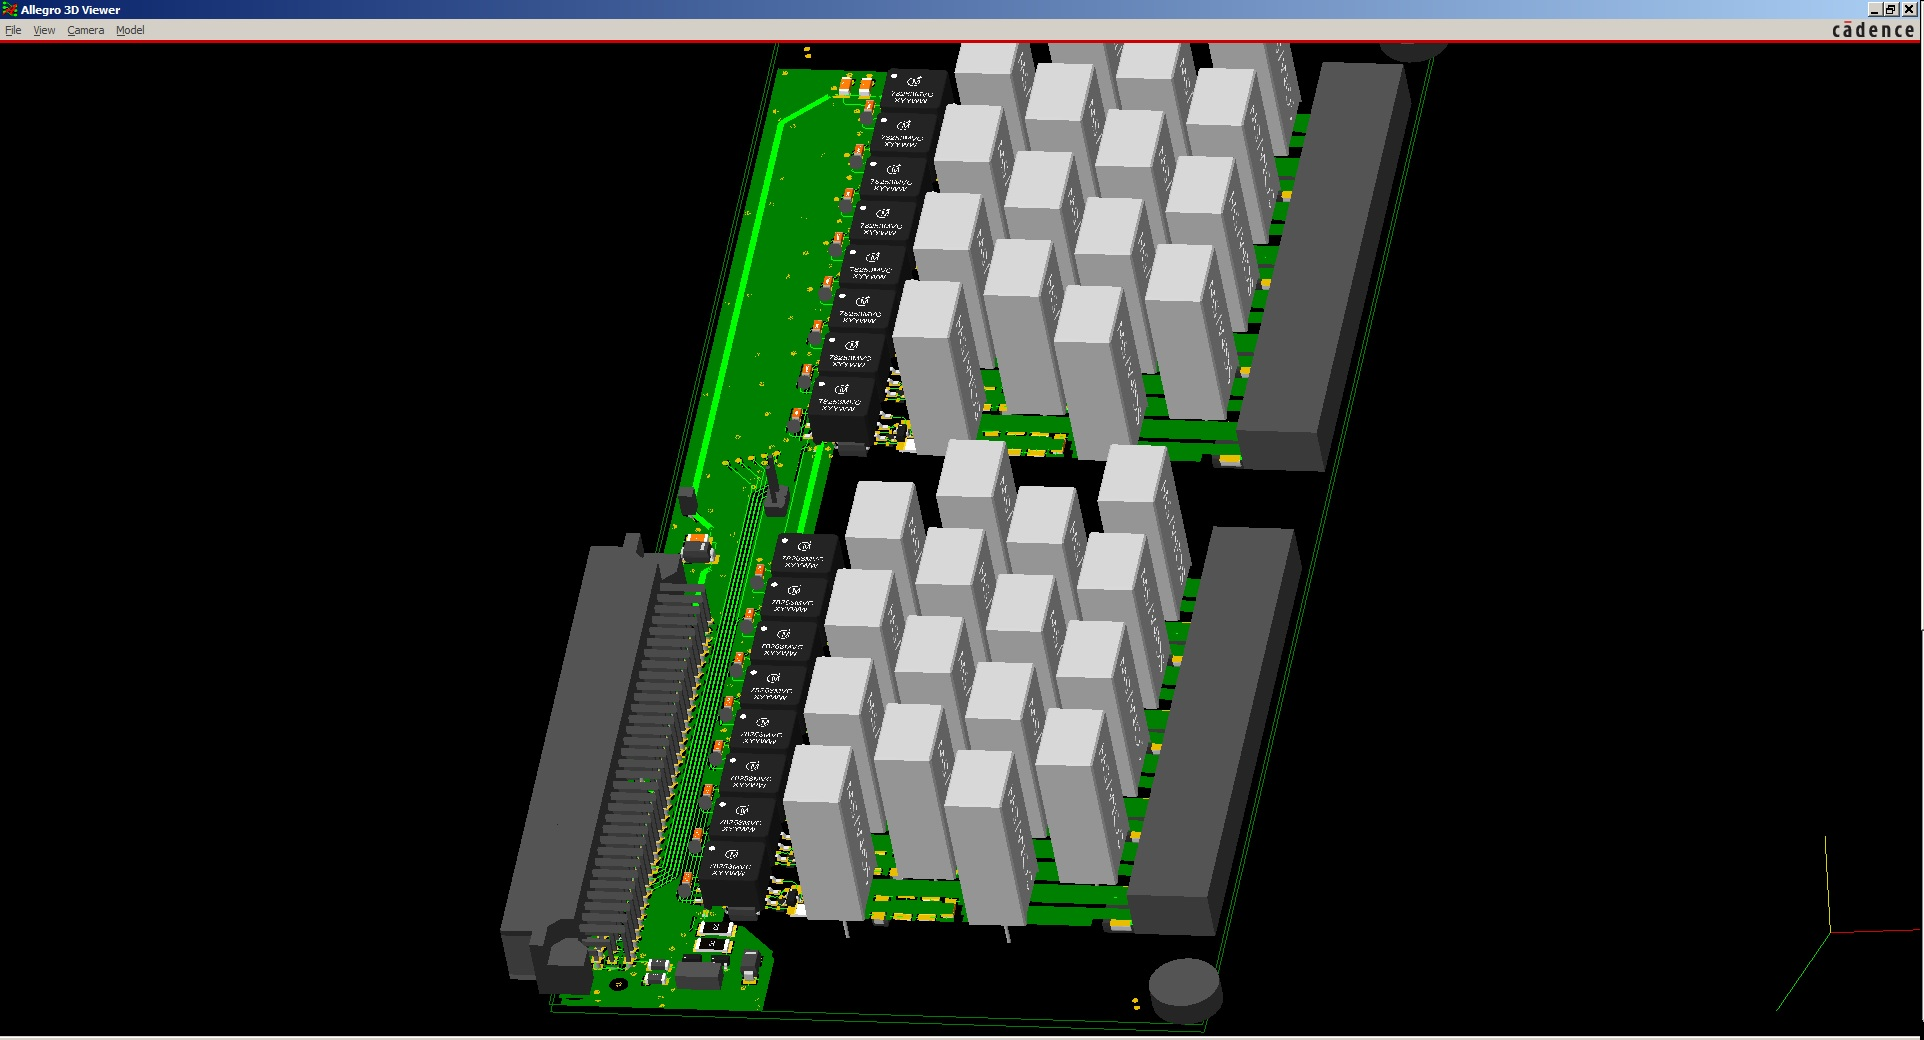
\includegraphics[width=0.8\linewidth]{example_3d_pcb.jpg}}
%		\caption{Пример платы с 3D моделями элементов} 
%		\label{fig:example_3d_pcb}
	\end{figure}
\end{enumerate}



%%-------
\newpage
\subsection{Надстройки} \label{ssec:pcb_plugin}



%%%-------
\subsubsection{Подключение} \label{sssec:pcb_plugin_setup}

Для подключения надстроек в~\textbf{PCB Editor} необходимо:
\begin{enumerate}
	\item Скопировать файлы в~папку \textit{<<\%CDS\_SITE\%/pcbenv/pcb/skil>>};
	\item Добавить загрузку надстроек в~файл \textit{allegro.init.txt} находящийся в той~же папке (либо создать его);
	\item В~зависимости от~надстройки, строка загрузки может принимать разный вид и необходимо ознакомиться с~приложенной к~ней документацией. Например, для \textbf{nsware} необходимо выполнить следующие действия:
	\begin{figure}[H]
		\center{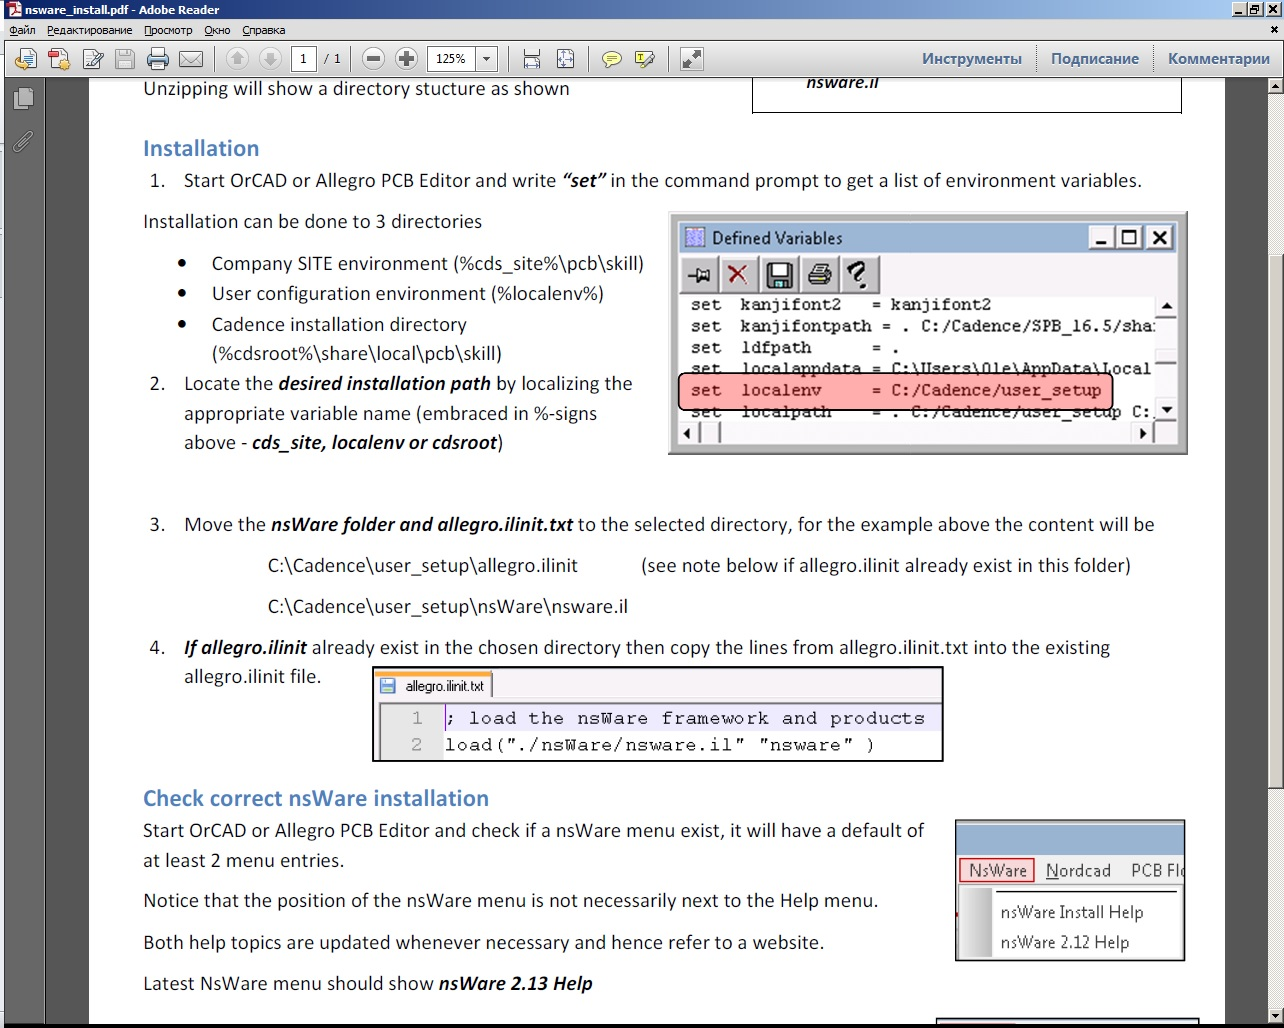
\includegraphics[width=0.8\linewidth]{nsware_plugin.jpg}}
%		\caption{Пример платы с 3D моделями элементов} 
%		\label{fig:example_3d_pcb}
	\end{figure}
	
	
	 
%%-------
\newpage
\subsection{Горячие кнопки} \label{ssec:hot_keys}
	 
Примеры горячих кнопок можно посмотреть в приложении \ref{app:hot_keys}.
	 
	 
	 
%%-------
\newpage
\subsection{Импорт и экспорт} \label{ssec:pcb_import}

\subsubsection{IPF файл}

По-умолчанию точка привязки при импорте и~экспорте данного формата располагается в~нижнем левом углу. Для удобства можно использовать точку привязки проекта установив флаг \textit{User Prefernces/ Manufacture/ Plot/ lp\_abs\_origin}.
	 
\end{enumerate}

\section{Pad Designer} \label{sec:pad_designer}

\ESKDappendix{Справочное}{Рекомендуемые значения для полей БД} \label{app:bd}
\begin{tabularx}{\linewidth}{|M{1.2cm}|X|M{1.7cm}|M{1.7cm}|M{1.7cm}|M{1.7cm}|}	
	\caption{Рекомендуемые значения поля \textit{Part Type} для \textbf{БД}} \label{tab:app_bd_part_type} \\
	
	\hline
    Адрес	& \calign{Название и~описание параметра}	& Масш.	& Мин.	& Макс.	& Доступ	\\ \hline
    \endfirsthead
    
    \multicolumn{6}{r}{продолжение следует\ldots} \\
    \endfoot
	\endlastfoot
	
	\multicolumn{6}{l}{Продолжение таблицы \ref{tab:app_bd_part_type}} \\ \hline 	
	Адрес	&  \calign{Название и~описание параметра} 	& Масш.		& Мин.		& Макс.		& Доступ	\\ \hline
	\endhead
	
	\multicolumn{6}{|c|}{Дата и~время} 																	\\ \hline
	1 		& Год 										& 1~год 	& 0 		& 99 		& чт./зап.	\\ \hline
	2 		& Месяц 									& 1~мес 	& 1 		& 12 		& чт./зап.	\\ \hline
    3 		& День 										& 1~день	& 1 		& 31 		& чт./зап.	\\ \hline
    4 		& Часы 										& 1~час 	& 0 		& 23 		& чт./зап.	\\ \hline
    5 		& Минуты 									& 1~мин 	& 0 		& 59 		& чт./зап.	\\ \hline
    6 		& Секунды	 								& 1~сек 	& 0 		& 59 		& чт./зап.	\\ \hline
\end{tabularx}

\begin{tabularx}{\linewidth}{|M{1.2cm}|X|M{1.7cm}|}	
	\caption{Рекомендуемые значения поля \textit{Case} для \textbf{БД}} \label{tab:app_bd_case} \\
	
	\hline
	Адрес	& \calign{Название и~описание параметра}	& Доступ	\\ \hline
	\endfirsthead
	
	\multicolumn{3}{r}{продолжение следует\ldots} \\
	\endfoot
	\endlastfoot
	
	\multicolumn{3}{l}{Продолжение таблицы \ref{tab:app_bd_case}} 	\\ \hline 
	Адрес	& \calign{Название и~описание параметра}	& Доступ	\\ \hline
	\endhead
	
	\multicolumn{3}{|c|}{Флаги текущего состояния} 					\\ \hline
	201 	& Неисправность 							&  чт. 		\\ \hline
	202 	& Предупреждение 							&  чт.		\\ \hline
	203		& Индикация команд передатчика				&  чт./зап.	\\ \hline
	204 	& Индикация команд приемника 				&  чт./зап.	\\ \hline 	
\end{tabularx}

\ESKDappendix{Справочное}{Примеры горячих кнопок для \textbf{PCB Editor}} \label{app:hot_keys}
\begin{tabularx}{\linewidth}{|X|m{6cm}|}	
%	\caption{} \label{} \\
	
	\hline
    \calign{Команда}	& \calign{Описание}	\\ \hline
    \endfirsthead
    
    \multicolumn{2}{r}{продолжение следует\ldots} \\
    \endfoot
	\endlastfoot
	
	\multicolumn{2}{l}{Продолжение таблицы} \\ \hline 	
	\calign{Команда}	& \calign{Описание}	\\ \hline
	\endhead
	
	
	\textit{funckey Esc cancel}		& Отмена действия по нажатию \textbf{<<Esc>>}.	\\ \hline
	\textit{funckey r iangle 90} 	& Поворот на 90 градусов по нажатию \textbf{<<r>>}.	\\ \hline
    \textit{funckey " " "pop bbdrill -cursor"} 	& Поставить переходное отверстие по нажатию \textbf{<<пробел>>}.	\\ \hline    
    \textit{funckey x "pick\_to\_grid -cursor"}	& Добавить точку излома по нажатию \textbf{<<x>>}.	\\ \hline
    \textit{funckey Del "prepopup; pop dyn\_option\_select @:@Delete"}	& Удаление элемента по нажатию \textbf{<<Del>>}.	\\ \hline
    \textit{funckey m "pop mirror"}	& перенос элемента на другой слой по нажатию \textbf{<<m>>}.	\\ \hline
    
    \multicolumn{2}{|c|}{Смена шага сетки}	\\ \hline
    \textit{alias CF1 "define grid; FORM grid non\_etch non\_etch\_x\_grids 1.0; FORM grid non\_etch non\_etch\_y\_grids 1.0; FORM grid all\_etch all\_etch\_x\_grids 1.0; FORM grid all\_etch all\_etch\_y\_grids 1.0; FORM grid done"}	& Выбор шага сетки 1мм по нажатию \textbf{<<Ctrl+F2>>}.	\\ \hline
    \textit{alias CF2 "define grid; FORM grid non\_etch non\_etch\_x\_grids 0.5; FORM grid non\_etch non\_etch\_y\_grids 0.5; FORM grid all\_etch all\_etch\_x\_grids 0.5; FORM grid all\_etch all\_etch\_y\_grids 0.5; FORM grid done"}	& Выбор шага сетки 0.5мм по нажатию \textbf{<<Ctrl+F1>>}.	\\ \hline
    \textit{alias CF5 "define grid; FORM grid non\_etch non\_etch\_x\_grids 2.54; FORM grid non\_etch no\_etch\_y\_grids 2.54; FORM grid all\_etch all\_etch\_x\_grids 2.54; FORM grid all\_etch all\_etch\_y\_grids 2.54; FORM grid done"}	& Выбор шага сетки 2.54 мм по нажатию \textbf{<<Ctrl+F5>>}.	\\ \hline
    \textit{alias CF6 "define grid; FORM grid non\_etch non\_etch\_x\_grids 1.27; FORM grid non\_etch non\_etch\_y\_grids 1.27; FORM grid all\_etch all\_etch\_x\_grids 1.27; FORM grid all\_etch all\_etch\_y\_grids 1.27; FORM grid done"}	& Выбор шага сетки 1.27 мм по нажатию \textbf{<<Ctrl+F6>>}.	\\ \hline
    
    \multicolumn{2}{|c|}{Смена толщины линии}																		\\ \hline
    \textit{funckey \textasciitilde1 'FORM mini acon\_line\_width Constrain' }	& Толщина линии согласно установленным ограничениям по нажатию \textbf{<<Ctrl+1>>}. . \\ \hline
    \textit{funckey \textasciitilde2 'FORM mini acon\_line\_width 0.2'} & Толщина линии 0.2мм по нажатию \textbf{<<Ctrl+2>>}.	\\ \hline
    \textit{funckey \textasciitilde7 'FORM mini acon\_line\_width 2.0'} & Толщина линии 2.0мм по нажатию \textbf{<<Ctrl+7>>}.	\\ \hline
    \textit{funckey w 'settoggle CMD \textasciitilde1 \textasciitilde2 \textasciitilde3 \textasciitilde4 \textasciitilde5 \textasciitilde6 \textasciitilde7;\textdollar CMD'} & Перебор заданных толщин линий по нажатию \textbf{<<w>>}	\\ \hline
    \multicolumn{2}{|c|}{Управление полигонами}	\\	
    \multicolumn{2}{|c|}{В \hyperlink{ssec:user_preferences}{my\_favorites} должен присутсвовать \textit{no\_shape\_fill}}	\\ \hline
    \textit{alias \textasciitilde k "enved; etchedit; setwindow form.prfedit; FORM prfedit next\_prfs; FORM prfedit no\_shape\_fill NO; FORM prfedit apply; FORM prfedit done; setwindow pcb"}	& Включение заливики полигонов по нажатию \textbf{<<Ctrl+"+"{} на~дополнительной клавиатуре>>}. \\ \hline
    \textit{alias \textasciitilde m "enved; etchedit; setwindow form.prfedit; FORM prfedit next\_prfs; FORM prfedit no\_shape\_fill YES; FORM prfedit apply; FORM prfedit done; setwindow pcb"}	& Отключение заливики полигонов по нажатию \textbf{<<Ctrl+"$-$"{} на~дополнительной клавиатуре>>}. \\ \hline
    
    \multicolumn{2}{|c|}{Смена подкласса}	\\ \hline
    funckey + subclass -+	& Смена текущего подкласса на стоящий ниже по списку по нажатию \textbf{<<+>>}. \\ \hline
    funckey - subclass --	& Смена текущего подкласса на стоящий выше по списку по нажатию \textbf{<<-->>}. \\ \hline
    funckey a altsubclass -+	& Смена подкласса перехода при постановке переходного отверстия по нажатию \textbf{<<a>>}.	\\ \hline
    funckey 1 options subclass TOP	& Выбор подкласса \textit{Top} по нажатию \textbf{<<1>>}.	\\ \hline
    funckey 4 options subclass BOTTOM	& Выбор подкласса \textit{Bottom} по нажатию \textbf{<<4>>}.	\\ \hline
    \multicolumn{2}{|c|}{Привязка}	\\ \hline
    \textit{funckey f "prepopup;pop dyn\_option\_select 'Snap pick to@:@Figure'"}	& Привязка к фигуре по нажатию \textbf{<<f>>}.	\\ \hline
    \textit{funckey i "prepopup;pop dyn\_option\_select 'Snap pick to@:@Intersection'"}	& Привязка к точке пересечения по нажатию \textbf{<<i>>}.	\\ \hline
    \textit{funckey c "prepopup;pop dyn\_option\_select 'Snap pick to@:@Arc/Circle Center'"}	& Привязка к центру дуги или круга по нажатию \textbf{<<c>>}.	\\ \hline
    \textit{funckey v "prepopup;pop dyn\_option\_select 'Snap pick to@:@Via'"}	& Привязка к переходному отверстию по нажатию \textbf{<<v>>}. \\ \hline
    
    \multicolumn{2}{|c|}{Настройки для колесика мышки}	\\ \hline
    button wheel\_up "roam y -\textdollar roamInc"	& Перемещение экрана вверх при вращении колесика \textbf{<<вверх>>}.	\\ \hline
    button wheel\_down "roam y \textdollar roamInc"	& Перемещение экрана вниз при вращении колесика \textbf{<<вниз>>}.	\\ \hline
    button SCwheel\_up "roam x \textdollar roamInc"	& Перемещение экрана вправо при вращении колесика \textbf{<<Shift+Ctrl+вверх>>}.	\\ \hline
    button SCwheel\_down "roam x -\textdollar roamInc"	& Перемещение экрана влево при вращении колесика \textbf{<<Shift+Ctrl+вниз>>}.	\\ \hline
    button Swheel\_up subclass -+	& Смена подкласса при вращении колесика \textbf{<<Shift+вверх>>}.	\\ \hline
    button Swheel\_down altsubclass -+	& Смена подкласса перехода при постановке переходного отверстия при вращении колесика \textbf{<<Shift+вниз>>}.	\\ \hline
    button Cwheel\_up zoom in	& Увеличение масштаба при вращении колесика \textbf{<<Ctrl+вверх>>}.	\\ \hline
    button Cwheel\_down zoom out	& Уменьшение масштаба при вращении колесике \textbf{<<Ctrl+вниз>>}.	\\ \hline
    
    
    
    
    	
\end{tabularx}

\begin{thebibliography}{9}
	\addcontentsline{toc}{section}{\refname}
	\bibitem{Connection Symbol Properties} FlowCAD, Application Note, Connection Symbol Properties. - 2013.
\end{thebibliography} \label{bib:bib}

\end{document}

